\section{Feature Learning}
The output of a parameterised DGN is given by:
\begin{align}
\hat{y}_t=\Phi_{\Tg_t}v_{\Theta_t},
\end{align}
which in comparison to \eqref{eq:fixednpf} has both the NPFs as well as the path values changing during training. As a result, the NTK matrix $K_t=K^v_t+K^{\phi}_t$ has two components: i) $K^v_t\in \R^{n\times n}$ captures the dynamics due to the flow of the value gradient through the corresponding active sub-networks, and ii) $K^{\phi}_t$ captures the dynamics due to the flow of feature gradient through the corresponding sensitive sub-networks. And under \Cref{assmp:main}, we know from \Cref{th:main}, that 
\begin{align*}
\E{K_0}=\mathbb{E}\big[K^v_0\big]+\E{K^{\phi}_0}=d\sigma^{2(d-1)} (x^\top x)\odot \lambda_0+\sigma^{2d}  (x^\top x)\odot \delta_0,
\end{align*}
where $\delta_0\in\R^{n\times n}$ is the correlation matrix of the sensitive sub-networks for the $n$ examples. Say in the case of classification with cross entropy loss, the gradient with respect to $\Tg$ will change the NPF matrix $\Phi_{\Tg_t}$ in such a manner to reduce the loss, i.e., increase the margin of each of the classified examples. Subject to the `well-conditioned' ness of $K^{\phi}_t$, such margin increase can be perhaps achieved for all the $n$ examples. To check our intuition on feature learning, we consider the following experiment on logistic regression with learnable features.\\
\begin{comment}
In the case of implicit parameterisation, i.e., when $\Tg=\Theta$, the NTK (see \Cref{tb:ntks}) is given by $K_t=K^v_t+K^{\phi}_t+{\Psi^{\phi}}^\top_t\Psi^v_t+ {\Psi^{v}}^\top_t\Psi^{\phi}_t$, where, in addition to $K^v_t$ and $K^{\phi}_t$, the other two terms occur due to the fact that the parameterisation is implicit. We now state the following theorem for the case of DGNs explicit parameterisation. A\begin{theorem}\label{th:main} Let $\delta(s,s')\stackrel{def}= \underset{{p\rsa i}}{\sum} \sum_{\tg\in\Tg}\frac{\partial A_{\Tg_0}(x_s,p)}{\partial \tg} \frac{\partial A_{\Tg_0}(x_{s'},p)}{\partial \tg}$, for $s,s'\in[n]$, using any $i\in[d_{in}]$. Then, under \Cref{assmp:main}, we have, $\E{K_0}=\mathbb{E}\big[K^v_0\big]+\E{K^{\phi}_0}$, where $\E{K^{v}_0}=d\sigma^{2(d-1)} (x^\top x)\odot \lambda_0$, and $\E{K^{\phi}_0}=\sigma^{2d}  (x^\top x)\odot \delta_0$.
\end{theorem}
\end{comment}
\begin{wrapfigure}{h}{0.25\textwidth}
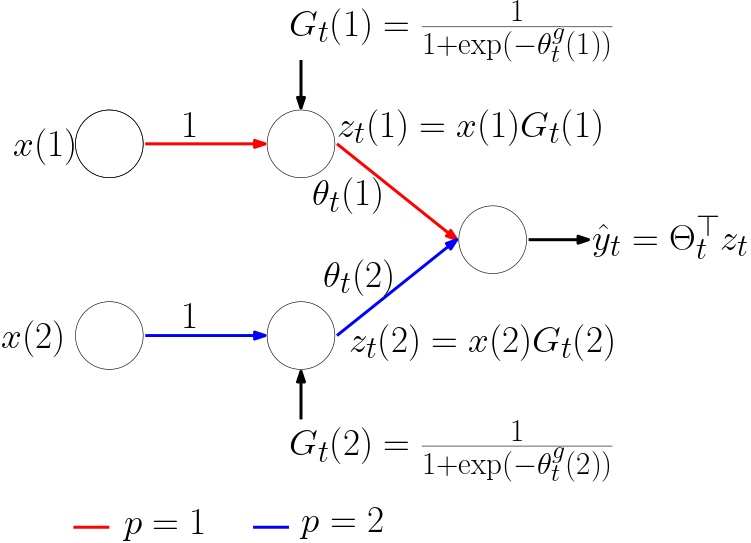
\includegraphics[scale=0.14]{figs/featlearn.png}
\caption{\label{fig:net}}
\end{wrapfigure}
\textbf{Logistic Regression with feature learning:} We look at a simple neural network in \Cref{fig:net} with $d_{in}=2$, $w=2$ and $1$-hidden layer. The first layer weights is an identity matrix, and for input $x\in\R^2$ to the network, the first layer output is given by $z_{t}(i)=x(i)G_t(i),i=1,2$, where $G_t(i)=\frac{1}{1+\exp(-\tg(i))},i=1,2$. In this network, there are $2$ paths, and the NPF is given by $\phi_{x,t}=(x(1)G_t(1),x(2)G_t(2))\in \R^2$. We check the performance of fixed-gates versus learnable gates in this network. We consider a binary classification task, with $n=500$ example for each class, with class $+1$ and $-1$  examples sampled from $U([0.1,1]\times [-a,a])$ and $U([-1,-0.1]\times[-a,a])$ respectively. \WFclear We considered two cases $a=1$ (first two plots from the left in \Cref{fig:feat}), and $a=100$ (right most plot in \Cref{fig:feat}). 
We trained the simple neural network using gradient descent with step-size of $0.1$, initialisation $\Tg_0=\Theta_0=(0,0)\in\R^2$, and binary cross entropy loss for the following two cases: i) fixed-gates, wherein, we set $\Tg_0=\Tg_t=\Tg_0,\forall t\geq 0$, and train only $\Theta_t$ ii) learnable gates, wherein, we train both $\Tg_t$ and $\Theta_t$. In all the plots, green bold and black dotted lines corresponds to classifier learned  by learnable and fixed gates respectively, and the points are represented using the NPF.\\
%While both cases train for $T=10^4$ epochs, for $T=10^3$ epochs only the model with adaptable gates trains successfully. The results are shown in \Cref{fig:feat}, notice that the right most plot shows that in the case when the gates are adapting, they learn to suppress the second co-ordinate (the scale of $\phi_{x_s,T}$ is from $-15$ to $15$ as opposed to $-100$ to $100$ in $x_s$).
\begin{figure*}[!t]
%\begin{minipage}{0.15\columnwidth}
%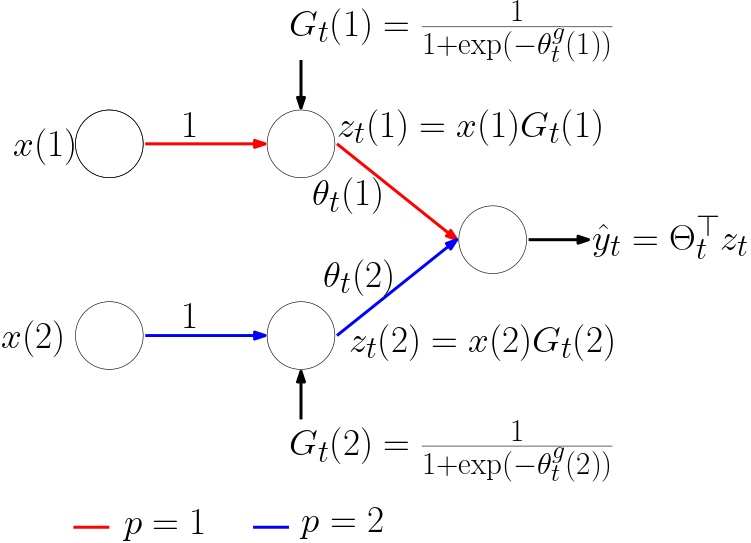
\includegraphics[scale=0.15]{figs/featlearn.png}
%\end{minipage}
%\hspace{50pt}
\begin{minipage}{1\columnwidth}
\resizebox{1\columnwidth}{!}{
\begin{tabular}{cccc}
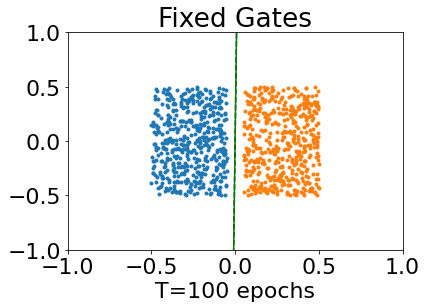
\includegraphics[scale=0.2]{figs/fixed-1e2-ae1.png}
&
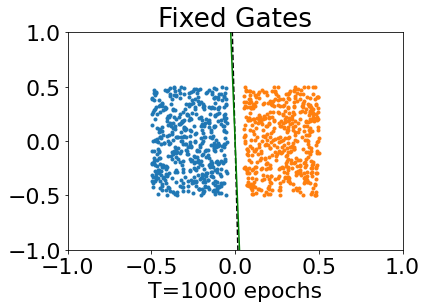
\includegraphics[scale=0.2]{figs/fixed-1e3-ae1.png}
&
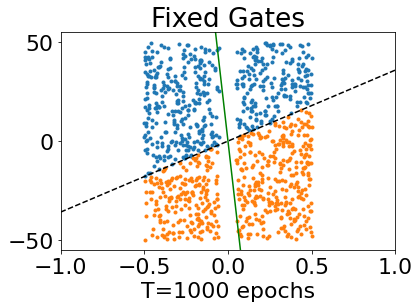
\includegraphics[scale=0.2]{figs/fixed-1e3-ae100.png}
&
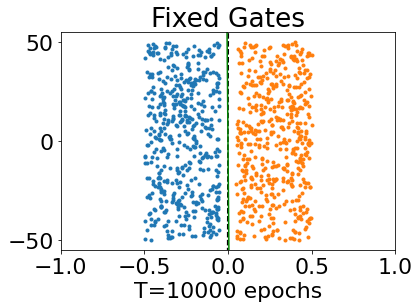
\includegraphics[scale=0.2]{figs/fixed-1e4-ae100.png}
\\
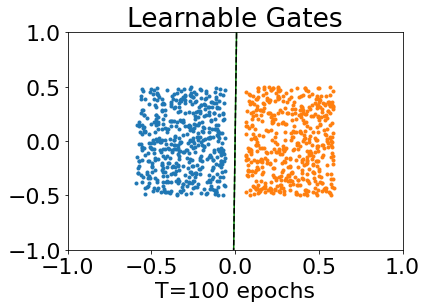
\includegraphics[scale=0.2]{figs/learn-1e2-ae1.png}
&
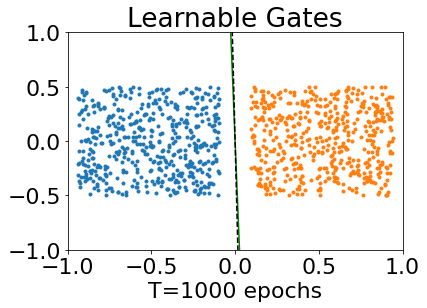
\includegraphics[scale=0.2]{figs/learn-1e3-ae1.png}
&
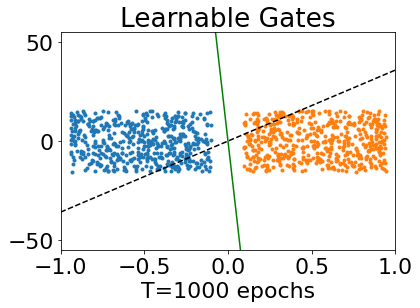
\includegraphics[scale=0.2]{figs/learn-1e3-ae100.png}
&
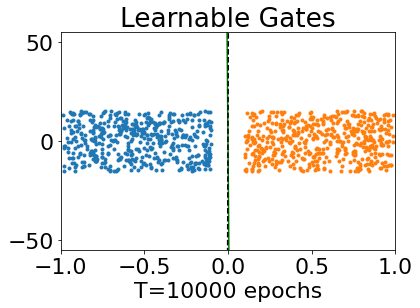
\includegraphics[scale=0.2]{figs/learn-1e4-ae100.png}
\end{tabular}
}
\end{minipage}

\caption{From left: second and third plots shows the training performance of fixed and learnable gates respectively. In both plots, the bold line in green is the classifier learnt in the case of learnable gates, and the dotted black line is the classifier learnt in the case of fixed gates. Notice the transformation of the feature space in the case of learnable gates.}
\label{fig:feat}
\end{figure*}
\textbf{Observations:}\\
$1.$ Initially for both networks $\tg_0=(0,0)^\top$, which means the horizontal and vertical co-ordinates in the NPF are both scaled by a factor of $0.5$. For the case of $a=1$, both networks train successfully in $T=10^2$ epochs, and we do not see any change in the NPFs. However, when trained for $T=10^3$ epochs, the network with learnable gates learns to scale the horizontal co-ordinate in the NPF by factor $1.0$, while it retains a value of $0.5$ for the vertical co-ordinate (see second plot from left of \Cref{fig:feat}).\\
$2.$ In the case of $a=100$ (right-most plot), the learnable network successfully trains in $T=10^3$ epochs by learning to scale the vertical co-ordinate down by a factor close to $0.15$. However, the network with fixed-gates does not train. We also observed that both networks trained successfully for $T=10^4$ epochs.
%\textbf{An open question:} Informally speaking, in the above example, even though the gating parameters had $2$-degrees of freedom, it was nonetheless sufficient to adapt the features. Thus, perhaps we can hypothesise that subject to the `well-conditioned' ness of $K^a_t$, such margin increase can be perhaps achieved for all the $n$ examples.  However, in practice, both $\Tg_t$ as well as $\Theta_t$ change, and an open question is to understand how the joint optimisation and feature learning happens. 

\begin{comment}
\textbf{Zeroth-order feature and kernel:} We now introduce the \emph{neural path feature} (NPF) and the \emph{neural path kernel} (NPK), which are zeroth-order quantities defined using the gating information $\G_t$. These quantities hold for all kinds of networks namely ReLU, GaLU, soft-ReLU and soft-GaLU. \\
The NPF of an input $x\in \R^{d_{in}}$ is given by $\phi_{x,t}=(x(\I_0(p))A_t(x,p) ,p\in[P])\in\R^P$. By arranging the NPF of the $n$ input examples in a matrix $\Phi_t=\left[\phi_{x_1,t},\ldots, \Phi_{x_n,t}\right]$, we can express the predicted output of a DGN as: \begin{align}\label{eq:npfbasic}\hat{y}_t=\Phi_t^\top v_t,\end{align}
where, the value of the path $v_t$ is the equivalent of the so called \emph{weight-vector} in a standard linear approximation. 

The significance of the NPF are:\hfill\\
$1.$ \textbf{Signal-Wire Separation}: Note that $\Phi$ encodes the signal: say for a DNN with ReLU activations, the co-ordinate corresponding to path $p$ is either $x(\I_0(p))$ if the path is active for that input (i.e., $A_t(x,p)=1$) or $0$ if the path is inactive for that input  (i.e., $A_t(x,p)=0$). The value of the path thus encodes the \emph{wire}, i.e., the information contained in the weights of the network. \hfill\\
$2.$ \textbf{Deep Information Propagation:} The path view provides a novel way of looking at information propagation in DNNs, eschewing the conventional `layer-by-layer' expression for information flow.\hfill\\
$3.$ \textbf{Representation:} As a parallel to the standard linear approximation, the NPF can be regarded as the \emph{hidden feature} and $v_t$ as the weight vector.
\end{comment}
\begin{comment}
$\lambda_t(s,s')$ is to be understood as the measure of overlap of the sub-networks that are active for both the inputs $x,x'\in\R^{d_{in}}$. Note that the definition of $\lambda_t$ is independent of $i\in [d_{in}]$: owing to symmetry the same number of paths start from any given input node, and looking forward, the paths see exactly the same gates and gating values in the subsequent layers.

%\subsection{First-order feature and kernel}
\textbf{Activity Derivative:} For a path $p$, and an input $x\inrdin$ the derivative of its activity with respect to any weight is given by 
\begin{align}
\frac{\partial A_{t}(x,p)}{\partial \tg}= \sum_{l=1}^{d-1} \Big(\frac{\partial G_{x,\Tg_t}(l,\I_l(p))}{\partial \tg} \Big)\Big(\Pi_{l'\neq l} G_{x,\Tg_t}(l',I_{l'}(p))\Big)
\end{align}
\end{comment}
%Note that in \Cref{def:delta}, $\delta_t$ contains $\partial A_t(x,p)$ terms as opposed to $A_t(x,p)$ term in $\lambda_t$ defined in \Cref{def:lambda}.
